\chapter{Week}

    The work continues with \texttt{jupyros} development. For this week, the focus was on navigation or being able to set up a navigation stack for any robot. The goal is to be able to visualize everything involved with navigation inside JupyterLab, this includes any sensor streams, maps, path planning, etc.

\section{tf2 Broadcaster}

    Following the ROS tutorial examples, it was simple task to implement a tf2 broadcaster within Jupyter. As of now, additional widgets for tf2 broadcasters and listeners does not appear to bring any immediate benefits.

    % \begin{lstlisting}
% def handle_turtle_pose(msg, turtlename):
%     br = tf2_ros.TransformBroadcaster()
%     t = geometry_msgs.msg.TransformStamped()
    
%     t.header.stamp = rospy.Time.now()
%     t.header.frame_id = "world"
%     t.child_frame_id = turtlename
%     t.transform.translation.x = msg.x
%     t.transform.translation.y = msg.y
%     t.transform.translation.z = 0.0
    
%     q = tf_conversions.transformations.quaternion_from_euler(0, 0, msg.theta)
%     t.transform.rotation.x = q[0]
%     t.transform.rotation.y = q[1]
%     t.transform.rotation.z = q[2]
%     t.transform.rotation.w = q[3]
    
%     br.sendTransform(t)
%     \end{lstlisting}

\section{Panda Transforms}

    As mentioned last week, Zethus is capable of displaying \texttt{tf} data. This was tested with Franka Emika's panda robot as seen in Figure \ref{fig:panda}. A few issues were encountered when trying to publish the robot description, this was because the \texttt{panda\_arm\_hand.urdf} was renamed to \texttt{panda\_arm.urdf} but this was fixed within the launch file.

\begin{figure}[H]
    \centering
    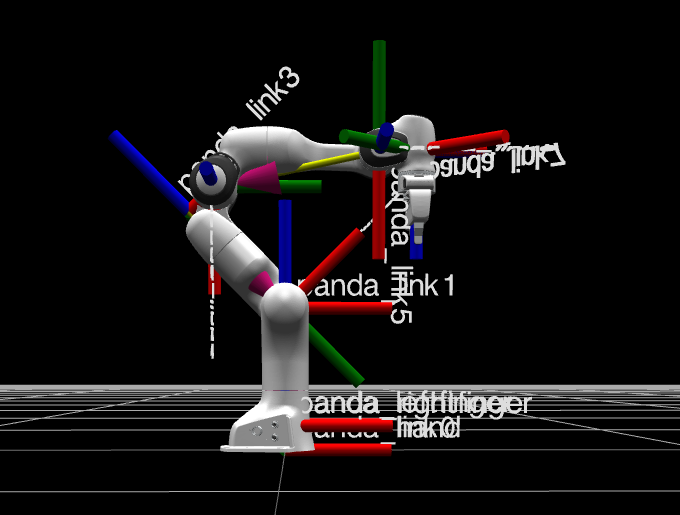
\includegraphics[width=0.6\linewidth]{Images/04_panda2.png}
    \caption{Transformations of Franka Emika's panda robot as displayed by Zethus}
    \label{fig:panda}
\end{figure}


\section{Interactive Markers}

    An example for using for using interactive markers and displaying them as a Jupyter widget was already included in the \texttt{jupyros} repository. However, this notebook used a \href{https://github.com/RobotWebTools/interactive_marker_proxy}{\texttt{interactive\_marker\_proxy}} package which was archived by the authors. Thus, the package had to be built from source and following the suggestions of Witalij Siebert's \href{https://github.com/RobotWebTools/interactive_marker_proxy/pull/4}{pull request}, the package was adapted to work with \texttt{tf2} and be compatible with ROS noetic.

    \begin{figure}[H]
            \centering
            \begin{subfigure}{.5\textwidth}
                \centering
                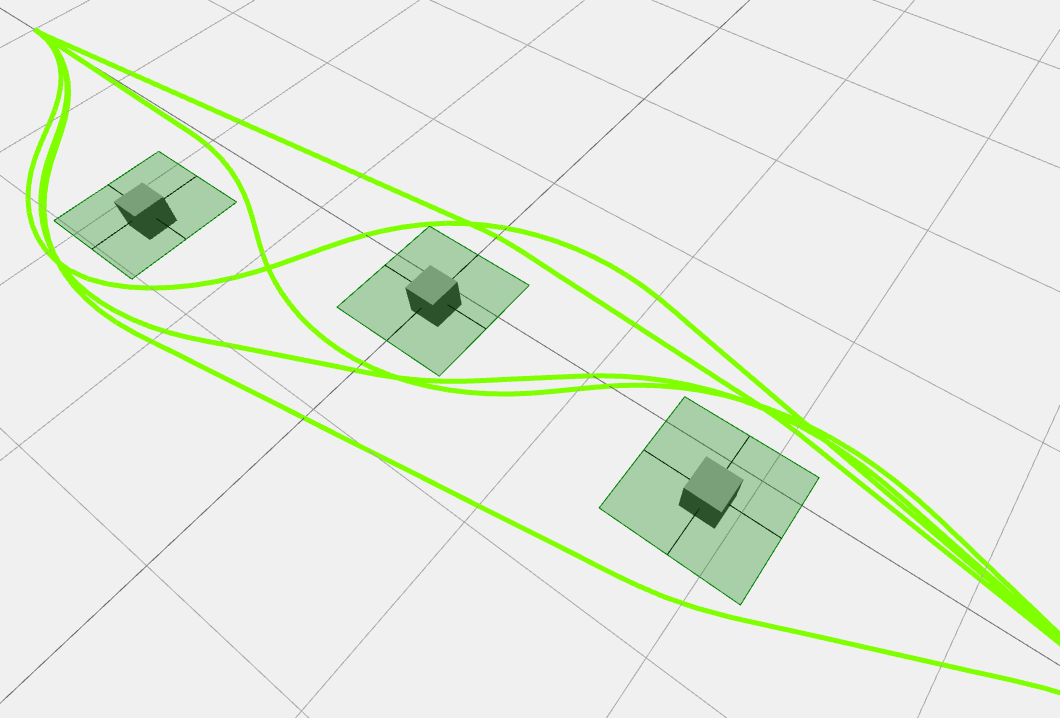
\includegraphics[height=5.7cm]{Images/04_markersZethus.png}
                \caption{Zethus display}
                \label{fig:markerRViz}
            \end{subfigure}%
            \begin{subfigure}{.5\textwidth}
                \centering
                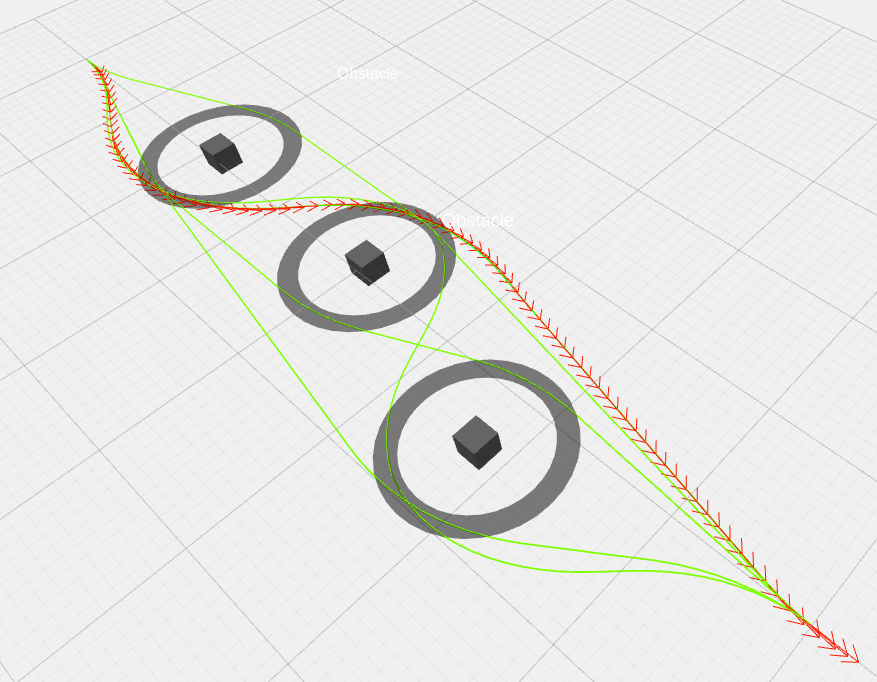
\includegraphics[height=5.7cm]{Images/04_markersRViz.png}
                \caption{RViz display}
                \label{fig:markerZethus}
            \end{subfigure}
            \caption{Interactive markers}
            \label{fig:markers}
    \end{figure}
    
    As illustrated in Figure \ref{fig:markerZethus}, Zethus is capable of representing the interactive markers and the possible paths. These markers can be easily moved with the mouse. The Zethus display can be compared to the RViz display of the same markers in Figure \ref{fig:markerRViz}. Currently there is no synchronization between Zethus and RViz, in other words, if one of the markers is moved to a new position in Zethus that new position will not be reflected in RViz and vice versa. However, synchronization may not be necessary because at the moment Zethus is meant to act as an RViz replacement.


\section{Laser Scanner}

    To prepare for the addition of sensors to the simulation, the ability of Zethus to display laser scans was examined. Without access to a live laser scanner, a \textit{fake} scanner was created. The generated fake scan can be observed in Figure \ref{fig:laser}. The size of the points here is exaggerated for display purposes, but this along other attributes can be directly modified with Zethus.

\begin{figure}[H]
    \centering
    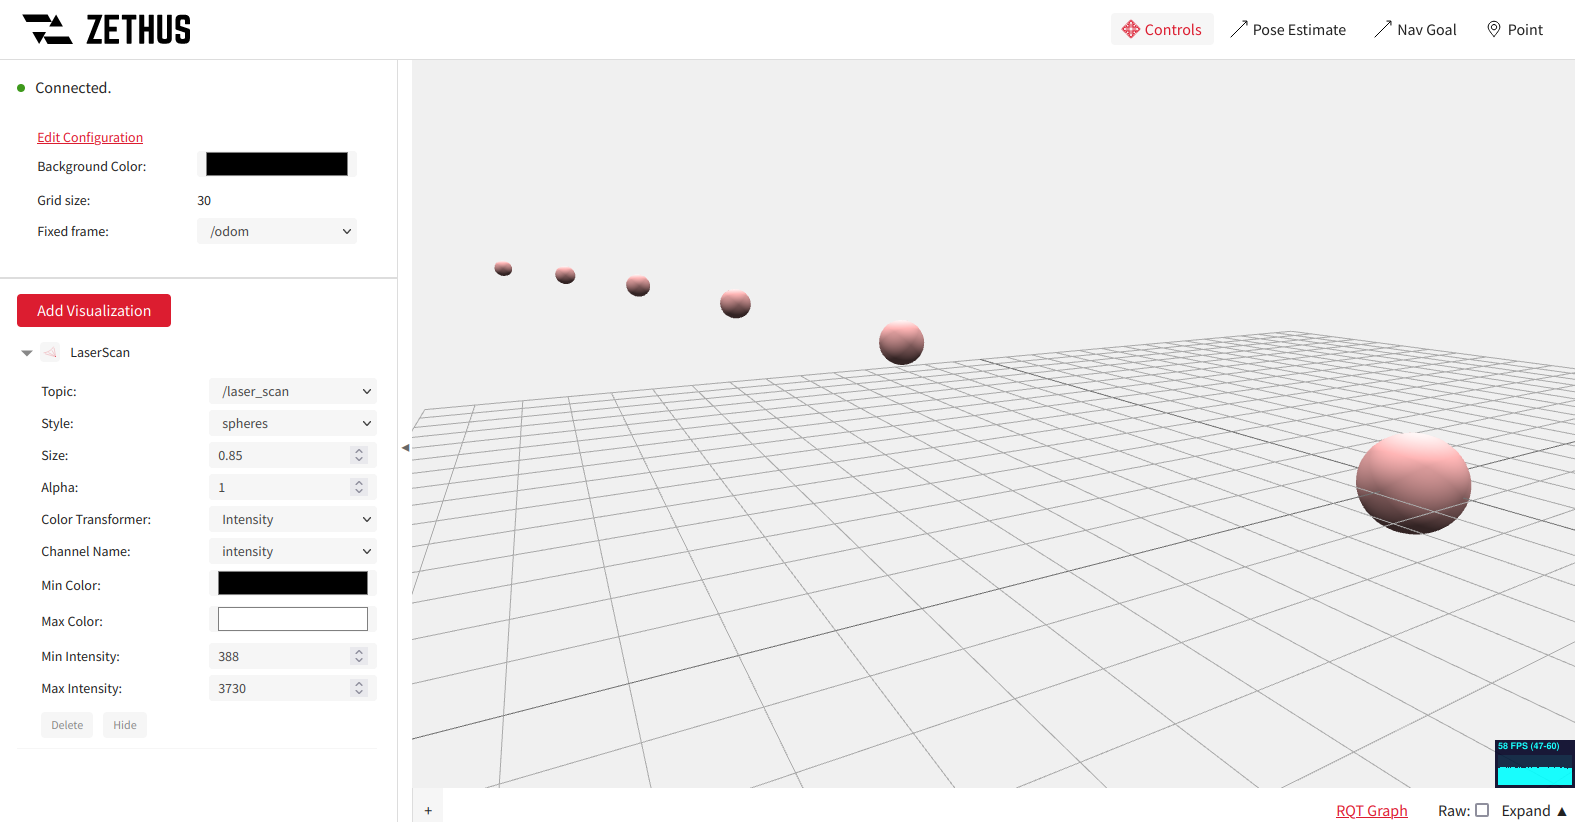
\includegraphics[width=\linewidth]{Images/04_laser.png}
    \caption{Display of a fake laser scan with Zethus}
    \label{fig:laser}
\end{figure}


\section{Gazebo}

    Since robot simulations are an essential part of the robotics ecosystem, adding support for a \href{https://gazebosim.org/home}{Gazebo} simulator became the next logical step. Fortunately, a web client for Gazebo has already been developed by Open Robotics which is called \href{https://github.com/osrf/gzweb}{GzWeb}. The functionality of this web simulator needed to be tested to determine if it could augment the capabilities of \texttt{jupyros}. 
    
    The testing process began by installing and building GzWeb. Initially there were a few issues with the build, but these were resolved by installing the missing dependencies and the supported versions of \texttt{nodejs} and \texttt{npm}. Afterwards, GzWeb ran as expected on a web browser.
    
    The next step was to display different world models to test the limitations of GzWeb. From this it was discovered that some colors and textures are not displayed correctly when compared to the classic Gazebo simulator; this issue requires further investigation. Figure \ref{fig:underwater} shows a simulation of an underwater world displayed in a web browser.
    
    A few additional issues were encountered during testing, mainly involving the left panel. When the light gray buttons are pressed to add more models or display the tree view, the entire panel disappears. 

\begin{figure}[H]
    \centering
    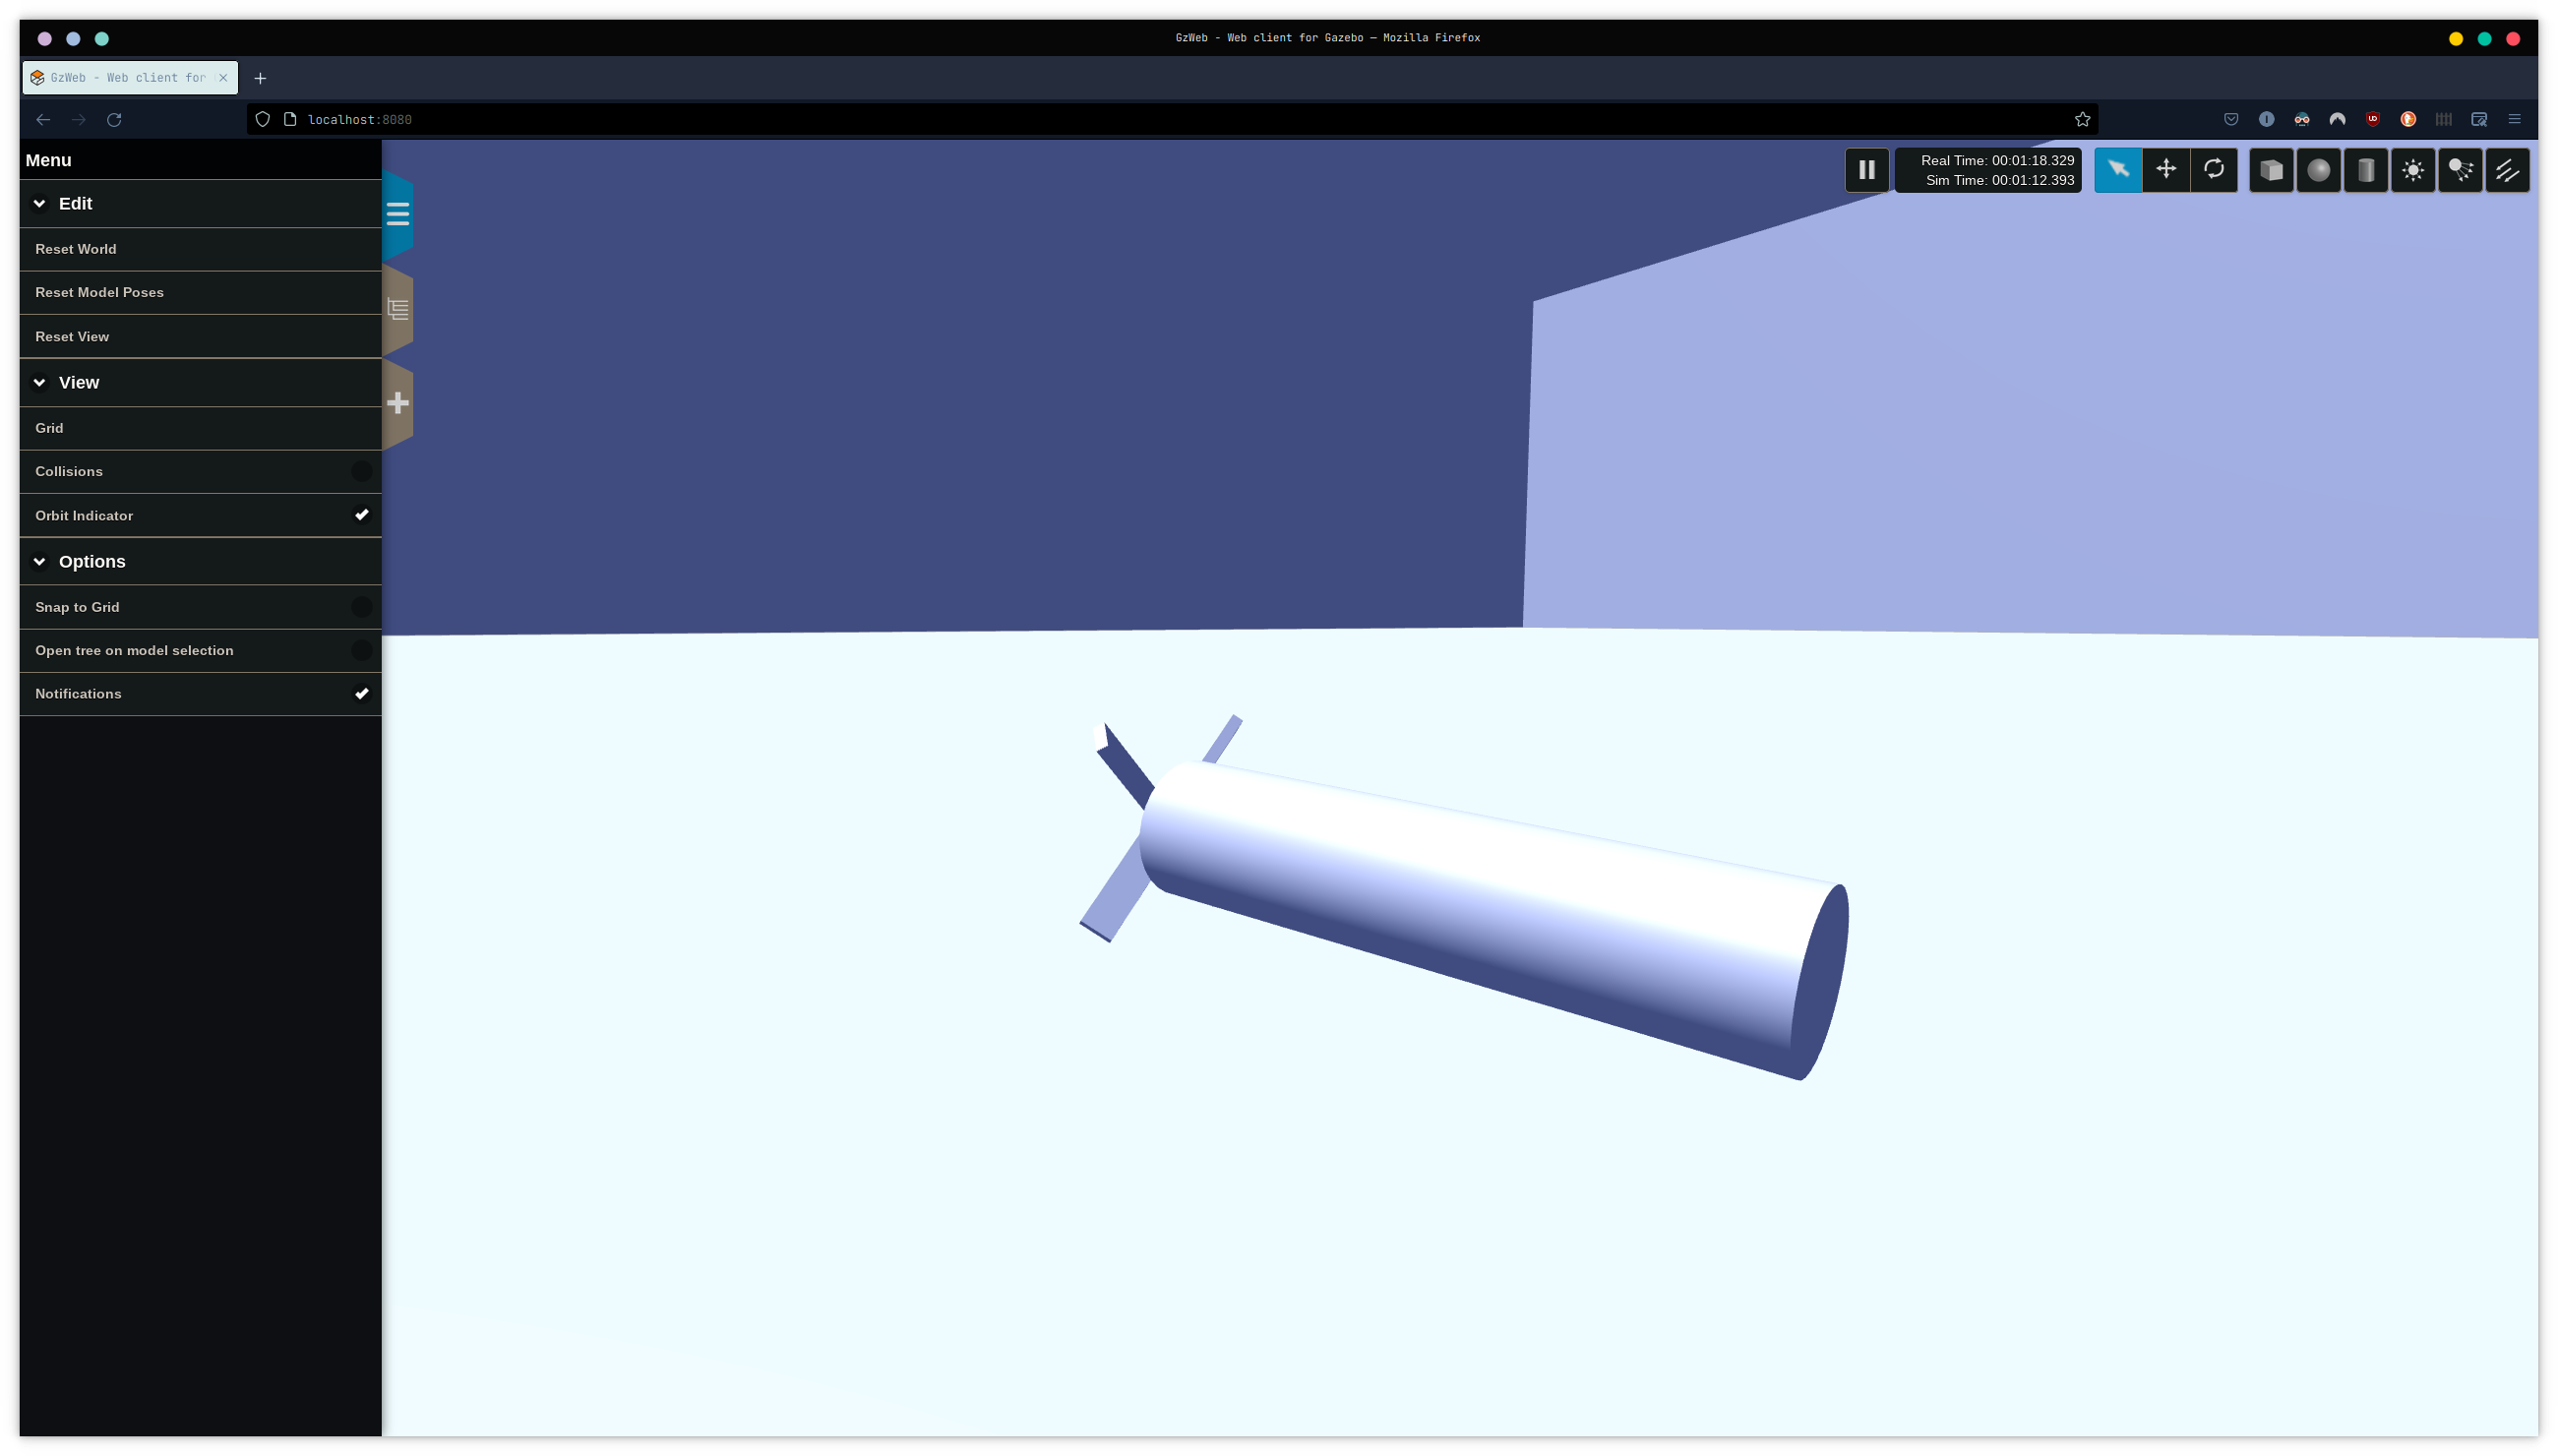
\includegraphics[width=\linewidth]{Images/04_underwater.png}
    \caption{Display of an \href{https://github.com/osrf/gazebo/blob/gazebo11/worlds/underwater.world}{underwater world} with Gazebo's web client}
    \label{fig:underwater}
\end{figure}


\section{Future Work}

    Zethus provides other visualization options such as image streams, maps, and point clouds. The limitations of these visualization types needs further exploration.

    Similarly, GzWeb also requires more investigation; the display issues can probably be solved by configuring the resource paths correctly. Additionally, some form of communication between GzWeb and the Jupyter ROS environment needs to be established in order to simulate robots which are managed from within a Jupyter notebook. And as a final step, GzWeb needs to be integrated into JupyterLab in the same manner that Zethus is integrated.